\chapter{Introduction to Faster-Than-Light Travel}

\section{Relativity? Who Cares?}
This section, while highly provocative, is quite small, and leaves something to be desired. Importantly, you can see that sections run together and do not cause page breaks like chapters do.

\section{Algorithms for Attempting the Leap Outside}
There are many ways to divide your paper down into a logical structure. Lets take a look at this in depth.

\subsection{No, Really, It's Totally Possible}
"In depth" was intended quite literally actually. The depth increases as we move into subsections like this one. Surprisingly we aren't done yet, though.

\subsubsection{Some Fine Details}
Do people really need sub-sub-sections? Well if you do, then here is how it will look.

\section{Math and Figures Look Nice}
Did you know math could look so fun? The dielectric constant at the air-metal interface
determines the resonance shift as absorption or capture occurs.

\begin{equation}
k_1=\frac{\omega }{c({1/\varepsilon_m + 1/\varepsilon_i})^{1/2}}=k_2=\frac{\omega
sin(\theta)\varepsilon_{air}^{1/2}}{c}
\end{equation}

\noindent
where $\omega$ is the frequency of the plasmon, $c$ is the speed of
light, $\varepsilon_m$ is the dielectric constant of the metal,
$\varepsilon_i$ is the dielectric constant of neighboring insulator,
and $\varepsilon_{air}$ is the dielectric constant of air.

% Example table to be displayed in the table list
\begin{table}[h]
    \begin{center}
        \begin{tabular}{|c|c|c|}
            \hline
            Column One & Column Two & Column Three \\ \hline
            a          & b          & c            \\ \hline
            1          & 2          & 3            \\ \hline
            x          & y          & z            \\ \hline
        \end{tabular}
    \end{center}
    \label{table:table1}
    \caption{Some Interesting Data Set}
\end{table}

% Example figure to be displayed in the figure list. pgfplots works nicely for generating graphs
\begin{figure}[h]
    \begin{center}
        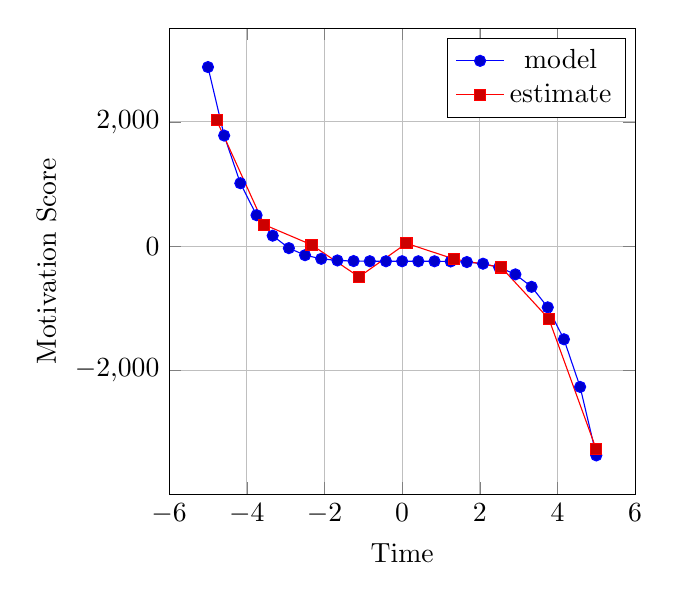
\begin{tikzpicture}
        	\begin{axis}[
        		height=7.5cm,
        		width=7.5cm,
        		grid=major,
        		ylabel=Motivation Score,
        		xlabel=Time
        	]
            	\addplot {-x^5 - 242};
            	\addlegendentry{model}
            
            	\addplot coordinates {
            		(-4.77778,2027.60977)
            		(-3.55556,347.84069)
            		(-2.33333,22.58953)
            		(-1.11111,-493.50066)
            		(0.11111,46.66082)
            		(1.33333,-205.56286)
            		(2.55556,-341.40638)
            		(3.77778,-1169.24780)
            		(5.00000,-3269.56775)
            	};
            	\addlegendentry{estimate}
        	\end{axis}
        \end{tikzpicture}
    \end{center}
    \label{figure:figure1}
    \caption{Thesis Writing Motivation Over Time}
\end{figure}
